\documentclass[aspectratio=169,t,11pt,table]{beamer}
\usepackage{../../slides,../../math}
\definecolor{accent}{HTML}{2B5269}
\definecolor{accent2}{HTML}{9D2235}

\title{Topic 2: Regression Toolkit}
\subtitle{\it  ECON 5783 — University of Arkansas}
\date{Fall 2024}
\author{Prof. Kyle Butts}

\begin{document}

% ------------------------------------------------------------------------------
\begin{frame}[noframenumbering,plain]
\maketitle

% \bottomleft{\footnotesize $^*$A bit of extra info here. Add an asterich to title or author}
\end{frame}
% ------------------------------------------------------------------------------

\begin{frame}{Linear Regression Bootcamp}
  This set of slides will serve as a `bootcamp' into one of the most popular tools in the applied researcher's toolkit: linear regression
  \begin{itemize}
    \item Creates a simple and interpretable model of $y$
    
    \item Has desirable properties for causal inference even if the outcome is not linear in covariates
  \end{itemize}
\end{frame}

\section{Conditional Expectation Function and Linear Model}


\begin{frame}{Prediction model}
  We have an outcome variable $y$ and a set of $p$ different predictor variables $X = (X_1, X_2, \dots, X_p)$. 
  \begin{itemize}
    \item For some observations we observe both $X$ and $y$; this is essential to \alert{fit} the model
  \end{itemize}

  \bigskip
  We can write the model in a general form as
  $$
    y = f(X) + \varepsilon,
  $$
  where $f$ is some unknown (but fixed) function of $X$. By definition $\varepsilon \equiv y - f(X)$ is the \alert{error term} that is needed to fit the data perfectly
\end{frame}

\begin{frame}{Prediction model}
  There are many different possible models of $f$ ranging from a linear model; a `smooth' model (polynomial or other); or a fully non-parametric function
\end{frame}

\imageframe{figures/f_examples_plot_raw.pdf}
\imageframe{figures/f_examples_plot_pred_1.pdf}
\imageframe{figures/f_examples_plot_pred_2.pdf}
\imageframe{figures/f_examples_plot_pred_3.pdf}
\imageframe{figures/f_examples_plot_pred_4.pdf}

\begin{frame}{Prediction model}
  There are many different possible models of $f$ ranging from a linear model; a `smooth' model (polynomial or other); or a fully non-parametric function
  
  \bigskip
  The more `fancy' a model:
  \begin{itemize}
    \item The more \alert{flexible} the relationship between $y$ and $X$ can be
    
    \item The larger the risk of \alert{overfitting} the data
    
    \item The less \alert{interpretable} the model becomes
  \end{itemize}
\end{frame}

\begin{frame}{Flexibility vs. Overfitting}
  \vspace{-\bigskipamount}
  \begin{center}
    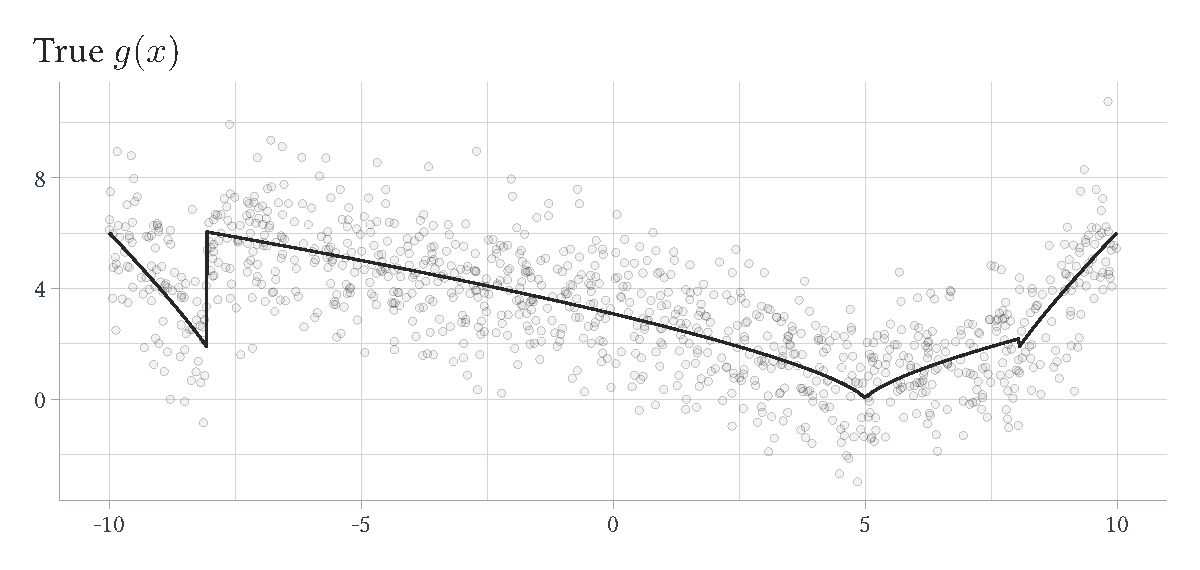
\includegraphics[width = \textwidth]{figures/f_examples_plot_dgp.pdf}
  \end{center}
\end{frame}

\begin{frame}{Flexibility vs. Overfitting}
  \vspace{-\bigskipamount}
  \begin{center}
    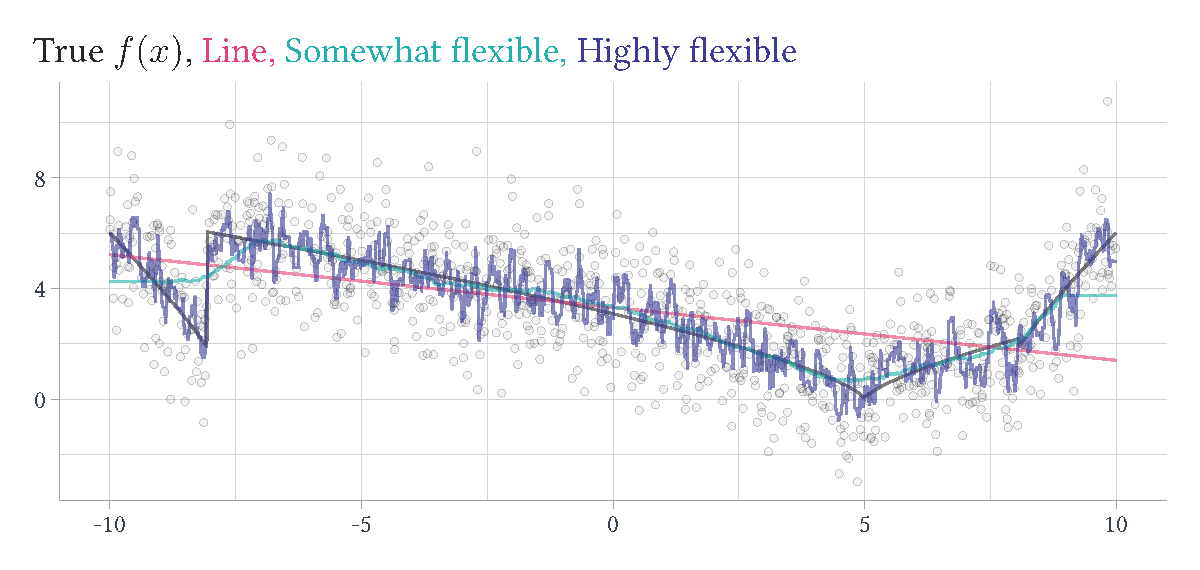
\includegraphics[width = \textwidth]{figures/f_examples_overfitting.pdf}
  \end{center}
\end{frame}

\begin{frame}{Flexibility vs. Overfitting}
  By making the model more and more \emph{flexible}, you risk overfitting more and more

  \begin{itemize}
    \item A solution is to evaluate your model fit using outside `testing data' (hold out some observations from fitting the model)
  \end{itemize}

  \pause
  \bigskip
  This technique is not as common when you care more about the associations between variables (interpreting the model)
  \begin{itemize}
    \item Not really a good reason other than "that is more complicated"
  \end{itemize}
\end{frame}


\subsection{Conditional Expectation Function}

\begin{frame}{The Conditional Expectation Function}
  In particular, we will think a lot about the \alert{Conditional Expectation Function} (CEF) of $y_i$ given $X_i = (X_{i1}, \dots, X_{ip})'$:
  $$
    g(x) \equiv \expec{y_i}{X_i = x}
  $$
  \begin{itemize}
    \item This reads ``$g(x)$ is the expected value of $y_i$ conditional on the unit having $X_i = x$''
  \end{itemize}

  \pause
  \bigskip
  The easiest way to estimate this for a given $x$ is to average $y_i$ for units with $X_i = x$. 
  \pause
  \begin{itemize}
    \item Only uses observations with $X_i = x$ (or $X_i \approx x$ when $X_i$ is continuous), so that is the relavent `$n$' when considering sample size
  \end{itemize}
\end{frame}

\imageframe{figures/f_examples_plot_dgp.pdf}
\imageframe{figures/f_examples_cef.pdf}

\begin{frame}{The Conditional Expectation Function}
  Uses of the conditional expectation function:
  \begin{enumerate}
    \item \alert{Descriptive}: how $y$ on average covaries with $X$ 
    \begin{itemize}
      \item By definition compare $g(x_1)$ to $g(x_2)$
    \end{itemize} 

    \item \alert{Prediction}: if we know $X_i$, our best guess for $y_i$ is $g(X_i)$ 
    \begin{itemize}
      \item Will prove `best guess' next
    \end{itemize} 
    
    \item \alert{Causal inference}: what happens to $y_i$ if we manipulate $X_i$ 
    \begin{itemize}
      \item Sometimes
    \end{itemize}
  \end{enumerate}

\end{frame}


\begin{frame}{Prediction Error and the CEF}
  The prediction error of the conditional expectation function is given by $\varepsilon_i = y_i - g(X_i)$. For any $x$, we have 
  \begin{align*}
    \expec{\varepsilon_i}{X_i = x} 
    &= \expec{y_i - \expec{y_i}{X_i = x}}{X_i = x} \\
    &= \expec{y_i}{X_i = x} - \expec{y_i}{X_i = x} \\
    &= 0
  \end{align*}
  
  \pause
  The prediction error is unpredictable given $X_i = x$
  \begin{itemize}
    \item We have \emph{used up} all the information that $X_i$ can give us. 
    \item This is not true for general $f(X)$
  \end{itemize}
\end{frame}

\begin{frame}{Mean-square prediction error}
  To provide a summary measure of fit, we want a `average' prediction error over the population
  \begin{itemize}
    \item If we took the average of prediction error, positive and negative prediction errors would cancel out
  \end{itemize}

  \pause
  \bigskip
  The \alert{mean-square (prediction) error} (MSE) for some model $f$ is calculated as:
  \begin{equation}\label{eq:mspe}
    \text{MSE}(f) \equiv \expec{\left( y_i - f(X_i) \right)^2}
  \end{equation}
  \vspace*{-\bigskipamount}
  \begin{itemize}
    \item Average over the population
  \end{itemize}
\end{frame}

\begin{frame}{Optimal model for $y$}
  The model $f$ that minimizes the mean-square prediction error is the conditional expectation function.
  \begin{align*}
    &\expec{\left( y_i - f(X_i) \right)^2} = \expec{\left( y_i - g(X_i) + g(X_i) - f(X_i) \right)^2} \\ \pause
    &\quad= \expec{\left( y_i - g(X_i) \right)^2} + \expec{\left( g(X_i) - f(X_i) \right)^2} + 2 \expec{\left( y_i - g(X_i) \right) \left( f(X_i) - g(X_i) \right)}
  \end{align*}

  \begin{itemize}
    \item The first term does not depend on $f$
  \end{itemize}
\end{frame}

\begin{frame}{Optimal model for $y$}
  The last term equals $0$: 
  \begin{align*}
    & \expec{\left( y_i - g(X_i) \right) \left( f(X_i) - g(X_i) \right)} \\
    &\quad= \expec{\expec{\left( y_i - g(X_i) \right) \left( f(X_i) - g(X_i) \right)}{X_i}} \\
    &\quad= \expec{\left( \expec{y_i}{X_i} - g(X_i) \right) \left( f(X_i) - g(X_i) \right)} \\
    &\quad= \expec{\left( g(X_i) - g(X_i) \right) \left( f(X_i) - g(X_i) \right)} \\
    &\quad= 0
  \end{align*}
\end{frame}

\begin{frame}{Optimal model for $y$}
  The model $f$ that minimizes the mean-square prediction error is the conditional expectation function.
  \begin{align*}
    &\argmin_{f} \expec{\left( y_i - f(X_i) \right)^2} = \expec{\left( y_i - g(X_i) + g(X_i) - f(X_i) \right)^2} \\
    &\quad= \argmin_{f} \expec{\left( y_i - g(X_i) \right)^2} + \expec{\left( g(X_i) - f(X_i) \right)^2} + 0
  \end{align*}

  \begin{itemize}
    \item Minimizing this with respect to $f$ only involves the second term so we set $f(X_i) = g(X_i)$
  \end{itemize}
\end{frame}

\begin{frame}{Optimal model for $y$}
  Therefore, in terms of mean-square prediction error, the conditional expectation function is the best predictor of $y$
\end{frame}

\subsection{Linear Model of Conditional Expectation Function}

\begin{frame}{Estimation of the CEF}
  As we discussed before, we could estimate $g(x) \equiv \expec{y_i}{X_i = x}$ by averaging over individuals with $X_i = x$
  \begin{itemize}
    \item In the case where $X_i$ is a discrete variable taking values $x_1, \dots, x_L$, this is just sub-sample averages for $X_i = x_\ell$
  \end{itemize}

  \pause
  \bigskip
  When $X_i$ is a multi-dimensional vector with many continuous variables, the density around any particular value $x$ is typically going to be small or near-zero 
  \begin{itemize}
    \item The so-called ``curse of dimensionality''
  \end{itemize}
\end{frame}

\begin{frame}{Linear Model}
  Instead, it is common to propose a \emph{parametric} model of the conditional expectation function:
  $$
    y_i = X_i' \beta + \text{error}
  $$
  \begin{itemize}
    \item We model $y$ as a linear function of the covariates
    \item Most of the time, we assume $X_i$ contains a constant for an intercept
  \end{itemize}

  \pause
  \bigskip
  Similar to the conditional expectation function, we can find the ``best'' linear predictor of $y$:
  $$
    \hat{\beta}_{\texttt{OLS}} \equiv \argmin_{\beta} \expec{\left( y_i - X_i' \beta \right)^2}
  $$
  \begin{itemize}
    \item Same as before but searching over only linear functions of $X$
  \end{itemize}
\end{frame}

\begin{frame}{Ordinary Least Squares}
  We can optimize this by taking first-order conditions and set equal to zero:
  \begin{align*}
    &\expec{ X_i \left( y_i - X_i' \beta_{\texttt{OLS}} \right) } = 0 \\
    &\implies \expec{ X_i y_i } - \expec{X_i X_i'} \beta_{\texttt{OLS}} = 0 \\
    &\implies \beta_{\texttt{OLS}} = (\expec{X_i X_i'})^{-1} \expec{ X_i y_i }
  \end{align*}

  \begin{itemize}
    \item The best linear predictor of $y$ is the ordinary-least squares estimate 
    
    \item Similar math shows $\beta_{\texttt{OLS}}$ is the best linear predictor of the CEF function $\expec{y_i}{X_i = x}$
  \end{itemize}
\end{frame}

\begin{frame}{Ordinary Least Squares Estimator}
  We can estimate using a sample of observations:
  $$
    \hat{\beta}_{\texttt{OLS}} = \left( \sum_{i=1}^n X_i X_i' \right)^{-1} \sum_{i=1}^n X_i y_i
  $$

  \bigskip
  Or in matrix notation
  $$
    \hat{\beta}_{\texttt{OLS}} = (X' X)^{-1} X' y
  $$
  \begin{itemize}
    \item $X$ is the $n \times k$ matrix with row given by $X_i'$ and $y$ is the column vector of outcome variables
  \end{itemize}
\end{frame}


\begin{frame}{Indicator Variables}
  When is a linear model of $g(x) \equiv \expec{y_i}{X_i = x}$ a good assumption?
  \begin{itemize}
    \item In some cases, the data might look to grow linearly in $X_i$, in which case, it is a reasonable assumption
  \end{itemize}

  \pause
  \bigskip
  A linear model means \emph{linear in parameters}; we can include polynomial terms to allow for non-linear (but smooth) model of $y_i$ given $X_i$
\end{frame}

\begin{frame}{Discrete variables}
  When $X_i$ is a discrete variable taking values $x_1, \dots, x_L$, consider a linear model consisting of a set of \alert{indicator variables} for each value of $x_\ell$:
  \begin{equation}\label{eq:dummy_variable_regression}
    y_i = \sum_{\ell = 1}^L \one{X_i = x_\ell} \beta_\ell + u_i
  \end{equation}
  \pause
  \begin{itemize}
    \item The ordinary least-squares estimator estimates $\hat{\beta}_{\ell} = \expechat{y_i}{X_i = x_\ell}$

    \pause
    \item In this case, the CEF is \emph{correctly specified} as the linear model (\ref{eq:dummy_variable_regression}).
  \end{itemize}
\end{frame}

\begin{frame}{Ommitted Categories}
  When we include a constant in the regression (or multiple sets of indicator variables) we have issues of \alert{multi-collinearity}:
  $$
    y_i = \alpha + \sum_{\ell = 2}^L \one{X_i = x_\ell} \beta_\ell + u_i
  $$

  We need to drop (at least) one of the indicator variables (say $\one{X_i = x_1}$). This serves as the ``reference category''
  $$
    \hat{\beta}_{\ell} = \expechat{y_i}{X_i = x_\ell} - \expechat{y_i}{X_i = x_1}
  $$
  \begin{itemize}
    \item $\hat{\beta}_{\ell}$ is the mean of group $\ell$ relative to the omitted group
  \end{itemize}
\end{frame}

\begin{frame}{Preview of Conditional Expectation Function usages}
  One main reason why we care about modeling $Y$ is because causal inference is a missing data problem
  \begin{itemize}
    \item For the treated units, we do not observe what their outcomes would be in the absence of treatment, $Y(0)$
    \item For the control units, we do not observe their $Y(1)$
  \end{itemize}

  \pause
  \bigskip
  If we fit a model for $\expec{Y_i(0)}{X_i = x}$, we can use this to make predictions for the treated units 
  
  \pause
  \begin{itemize}
    \item The model predicting out of sample for our treated group requires certain conditions we'll discuss in topic 3
  \end{itemize}
\end{frame}


\section{Omitted Variable Bias (OVB)}

\begin{frame}{Difference between true model and model we estimate}
  Say there is a true causal model for $y$
  $$
    y_i = \beta_0 + X_{i1} \beta_1 + X_{i2} \beta_2 + \varepsilon_i
  $$
  \begin{itemize}
    \item Assume $\expec{\varepsilon_i}{X_i} = 0$ so that $\beta_1$ is the true causal effect
  \end{itemize}
  
  \pause
  \bigskip
  But we only estimate a `short' regression specification
  $$
    y_i = \delta_0 + X_{i1} \delta_1 + error
  $$

  \bigskip
  What is the relationship between $\beta_1$ the true causal effect and the coefficient $\delta_1$?
\end{frame}

\begin{frame}{Omitted Variable Bias}
  \vspace*{-\bigskipamount}
  $$
    \underbrace{y_i = \beta_0 + X_{i1} \beta_1 + X_{i2} \beta_2 + \varepsilon_i}_{\text{``long regression''}} \quad\text{ and }\quad \underbrace{y_i = \delta_0 + X_{i1} \delta_1 + \text{error}_i}_{\text{``short regression''}}
  $$

  \bigskip
  We have the following relationship:
  \begin{align*}
    \delta_1 
    &= \frac{\cov(X_1, y)}{\var{X_1}} \\
    &= \frac{\cov(X_1, \beta_0 + X_{1} \beta_1 + X_{2} \beta_2 + \varepsilon)}{\var{X_1}} \\ \pause
    &= \beta_1 + \beta_2 \frac{\cov{X_1, X_2}}{\var{X_1}} 
  \end{align*}
\end{frame}

\begin{frame}{Omitted Variable Bias}
  $$
    \hat{\delta}_1 = \beta_1 + \beta_2 \frac{\cov{X_1, X_2}}{\var{X_1}} 
  $$

  \bigskip
  The reason this is true is due to regression being a prediction model!
  \begin{itemize}
    \item If $X_1$ and $X_2$ are correlated, then knowing about $X_1$ tells me information on $X_2$
    
    \item I would want to use that implicit information on $X_2$ to predict $y$ as well! 
  \end{itemize}

  \bigskip
  $\implies$ take the effect of $\beta_2$ times how I think $X_1$ tells me about $X_2$
\end{frame}

\begin{frame}{Omitted Variable Bias}
  $$
    \hat{\delta}_1 = \beta_1 + \beta_2 \frac{\cov{X_1, X_2}}{\var{X_1}} 
  $$

  \bigskip
  We can often times `sign' the bias:
  \begin{itemize}
    \item The sign of $\beta_2$ is what we think the effect of $X_2$ is on $y$
    \item $\cov{X_1, X_2}$ is how $X_1$ and $X_2$ are related in the population
  \end{itemize}
\end{frame}

\begin{frame}{Signing the Bias}
  \begin{center}
    \begin{tabular}{@{\extracolsep{5pt}} l | c | c | c}
      \toprule
                    & $\cov(X_1, X_2) > 0$ & $\cov(X_1, X_2) < 0$ & $\cov(X_1, X_2) = 0$ \\
      \midrule
      $\beta_2 > 0$ & positive bias        & negative bias  & no bias\\
      \midrule
      $\beta_2 < 0$ & negative bias        & positive bias  & no bias\\
      \midrule
      $\beta_2 = 0$ & no bias              & no bias        & no bias\\

      \bottomrule
    \end{tabular}
  \end{center}

  \bigskip
  If $X_2$ is unrelated to $X_1$ \emph{or} $X_2$ has no effect on $y$, then we have no problem
\end{frame}

\subsection{Reinterpreting selection bias as OVB}

\begin{frame}{Omitted Variable Bias}
  Let $X_1$ is an indicator variable, call it $D$. 
  \begin{align*}
    \cov{D, X_2} 
    &= \expec{ (D - \expec{D}) (X_2 - \expec{X_2})} \\
    &= \expec{D (X_2 - \expec{X_2})} \\
    &= \expec{X_2}{D = 1} - \expec{X_2}
  \end{align*}

  Let $\pi = \prob{D = 1}$ and note from definition, $\var{D} = \pi (1 - \pi)$. Then,
  $$
    \delta_1 = \beta_1 + \frac{\beta_2}{\pi (1 - \pi)} \left( \expec{X_2}{D = 1} - \expec{X_2} \right)
  $$
\end{frame}

\begin{frame}{Selection Bias}
  \vspace*{-\bigskipamount}
  $$
    \delta_1 = \beta_1 + \frac{\beta_2}{\pi (1 - \pi)} \left( \expec{X_2}{D = 1} - \expec{X_2} \right)
  $$

  \bigskip
  In our context of $D$ being a treatment indicator, $\delta_1$ is our treatment effect estimate and $\beta_1$ is the true ATT.

  \pause
  \bigskip
  We see that if the mean of $X_2$ differs for the treatment group, then our estimate is biased
  \begin{itemize}
    \item E.g. if $D$ is college attendance and $X_2$ is parental income, then our treatment effect is biased if college attendees have difference average parental income
  \end{itemize}
\end{frame}


\begin{frame}{OVB In Practice}
  A lot of research will run regressions that look like 
  $$
    y_i = D_i \tau + X_i' \beta + \varepsilon_i
  $$

  \bigskip
  The \emph{key things} you will want to do is think through what might show up in the error term
  \begin{enumerate}
    \item If those omitted variables are correlated with $D_i$ (after controlling for $X_i$) and have an effect on $y_i$, then you have problems interpreting the effect as causal
  \end{enumerate}
\end{frame}


\section{Frisch-Waugh-Lovell Theorem}

\begin{frame}{Projection Matrix}
  Before we describe the Frisch-Waugh-Lovell theorem, let's define a few terms. Consider our regression estimator
  $$
    \hat{\beta} = \left( X'X \right)^{-1} X' y
  $$
  
  \bigskip
  We could then create fitted values by multiplying $X$ by our coefficient of interest: 
  $$
    X \hat{\beta} = X \left( X'X \right)^{-1} X' y \equiv P_X y
  $$
  \begin{itemize}
    \item We define the \alert{Projection Matrix} as $P_X$ to be the fitted values from a regression of a variable on the variables $X$.
  \end{itemize}
\end{frame}

\begin{frame}{Residuals}
  The residuals from the regression are given by $\hat{\varepsilon} = y - \hat{y} = y - P_X y$

  \bigskip
  In matrix notation, we can write this as $\hat{\varepsilon} = (I - P_X) y$. We define $M_X$ to be the \alert{annihilator matrix} with $M_X \equiv I - P_X$

  \pause
  \begin{itemize}
    \item The annihilator matrix first predicts $y$ using a linear model of $X$ and then subtracts off the prediction
  \end{itemize}
\end{frame}

\begin{frame}{Residuals}
  From regression algebra we have the residuals are (linearly) uncorrelated with $X_i$ 
  $$
    \expec{X_i \hat{\varepsilon}_i} = 0
  $$
  
  \bigskip
  \pause 
  If we assume that the CEF $\expec{y_i}{X_i} = X_i' \beta$, then we can go further and say 
  $$
    \expec{\hat{\varepsilon}_i}{X_i = x} = 0
  $$
  \begin{itemize}
    \item the remaining variation in $y_i$, given by $\hat{\varepsilon}_i$, is unpredictable given $X_i$
  \end{itemize}
\end{frame}


\begin{frame}{Frisch-Waugh-Lovell Theorem}
  Consider the regression
  $$
    y_i = \tau D_i + W_i' \beta + u_i
  $$
  \begin{itemize}
    \item $D_i$ is a scalar variable of interest and $W_i$ is a $k \times 1$ vector of covariates
  \end{itemize}

  \bigskip
  We can of course estimate the regression coefficients $\hat{\tau}$ and $\hat{\beta}$ jointly in a single regression
\end{frame}

\begin{frame}{Frisch-Waugh-Lovell Theorem}
  The \alert{FWL theorem} shows that instead of doing one regression, we could estimate $\hat{\tau}_{\texttt{OLS}}$ by the series of steps:
  \begin{enumerate}
    \item Regress $y_i$ on $W_i$ and grab the residuals, $M_W y$
    \item Regress $D_i$ on $W_i$ and grab the residuals, $M_W D$
    \item Regress $M_W y$ on $M_W D$ to estimate $\hat{\tau}_{\texttt{FWL}}$
  \end{enumerate}

  \bigskip
  \pause
  The estimate $\hat{\tau}_{\texttt{FWL}}$ is going to be \emph{numerically identical} to $\hat{\tau}_{\texttt{OLS}}$.
  \begin{itemize}
    \item Up to degree-of-freedom correction, the standard errors will be identical as well (including robust and clustered standard errors)
    \begin{itemize}
      \item The final regression pretends we didn't estimate the $K$ coefficients on $W_i$
    \end{itemize}
  \end{itemize}
\end{frame}

\begin{frame}{Frisch-Waugh-Lovell Theorem}
  The FWL Theorem shows us how to think about the regression coefficient in a multivariate regression:
  \begin{itemize}
    \item We are predicting $D_i$ and $y_i$ using covariates $W_i$
    \item We are removing that predictable variation and seeing if the ``remaining variation'' in $y_i$ and $D_i$ are linearly correlated
  \end{itemize}

  \pause
  \bigskip
  To be clear, we do not have to run these regression; we can interpret our regression results as if we had run it using this procedure
\end{frame}

\begin{frame}{Example of Frisch-Waugh-Lovell Thinking}
  We want to know the causal effect of college on earnings
  \begin{itemize}
    \item $D_i$ is an indicator for a person going to college
    
    \item $y_i$ is the worker's earnings at age 25
    
    \item $W_i$ is a vector of covariates we think are important determinents of college attendance and/or earnings
  \end{itemize}

  Run this regression:
  $$
    y_i = \tau D_i + W_i' \beta + u_i
  $$

\end{frame}

\begin{frame}{Example of Frisch-Waugh-Lovell Thinking}
  The regression estimate will do the following:
  \begin{itemize}
    \item Predict whether a worker would go to college given the covariates $W_i$. The difference between $D_i$ and the prediction $\hat{D}_i$ is \emph{hopefully} due to random reasons
    
    \item Predict how those covariates $W_i$ would affect future earnings and remove that prediction. The remaining variation in wages is hopefully driven by (i) either college attendance, or (ii) other reasons that are uncorrelated with going to college
  \end{itemize}

  \bigskip
  It is important therefore to know a lot about your subject and know what causes treatment uptake $D_i$
\end{frame}

\begin{frame}{Example of Frisch-Waugh-Lovell Thinking}{College attendance}
  Like with omitted variable bias, this is a story of what variables did we not include. In our college attendance example, say $W_i$ is parental income and GPA. 
  \begin{itemize}
    \item Both are important drivers of college attendance, but not the only ones
  \end{itemize}

  \bigskip
  What are examples of other variables that can drive attendance?
\end{frame}



\section{More Flexible Approximations (\texttt{binscatter})}

\begin{frame}{Partially linear model}
  The \alert{Partially linear model} mixes high model flexibility in a key variable we care about and linear model for the rest of the covariates:
  $$
    y_i = \mu(X_i) + W_i' \beta + u_i
  $$
  \begin{itemize}
    \item $\mu(X_i)$ is a highly flexible function
    \item $W_i'$ is a set of \emph{linear} control variables
  \end{itemize}

  \bigskip
  This allows you to prevent the curse of dimensionality by linearly controlling for most of the variables. Allows a flexible model for the key variable of interest, $X_i$, that is good for graphing
\end{frame}

\begin{frame}{Partially linear model}
  $$
    y_i = \mu(X_i) + W_i' \beta + u_i
  $$
  One recent way of estimating this is using a `binscatter' regression 
  \begin{itemize}
    \item Raj Chetty and coauthors use this method a lot since they have too many observations for normal scatterplots
  \end{itemize}
\end{frame}

\begin{frame}{Binscatter Regression}
  $$
    y_i = \mu(X_i) + W_i' \beta + u_i
  $$
  One recent way of estimating this is using a `binscatter' regression:
  \begin{enumerate}
    \item Chop $X$ variable into $J$ bins with an equal number of observations into each bin
    
    \item Fit some polynomial of $X$ just within each bin (interact $X$ polynomial with bin indicators)
  \end{enumerate}
\end{frame}

\imageframe{figures/ex_binsreg_raw.pdf}
\imageframe{figures/ex_binsreg_split_into_bins.pdf}
\imageframe{figures/ex_binsreg_bins.pdf}
\imageframe{figures/ex_binsreg_bins_add_linear.pdf}
\imageframe{figures/ex_binsreg_bins_add_smooth.pdf}


% \section{Binary Outcome Variable}



\end{document}
